\chapter{介紹}
\section{研究目的與動機}

以往,玩射飛鏢需要有鏢靶跟飛鏢等器材,且受到空間限制,需在足夠大的空間讓玩家投擲飛鏢。本團隊希望創造不受空間,器材限制的射飛鏢手機遊戲。此次實作在Android手機上開發,使用者只需開起前鏡頭,達到不須攜帶任何物品,即可於各地遊玩飛鏢遊戲。且支援各種Android系統手機,可用度廣泛。
為達成不受器材之限制,使用擴增實境技術,將虛擬飛鏢、虛擬鏢靶呈現於遊戲畫面中,且在發射過程中,能繪製出發射的過程,達到擬真的效果;另外,需具備高即時性,能在比出發射飛鏢之手勢後,能立即偵測使用者是否發射以及力度,達到實際發射飛標的情況,而此我們將使用神經網路以及串流的技術來達成。
總結以上,本研究著重於如何將虛擬實境的射飛鏢更貼近實際發射飛鏢的體驗,且藉由本次實作,探討神經網路、特徵點辨識、即時傳輸之技術。


\section{系統簡介(遊戲說明、流程圖、多人運作)}

本系統為使用 Augmented Reality 與 Deep Learning 技術結合而成的射飛鏢遊戲。手機端部分 (Client) 偵測由我們所設計的特殊標定物,將標定物放置於牆面,手機後相機對準標定物,左右移動相機角度,手機即會顯示鏢靶於該標定物上,同時,飛鏢便會顯示於手機螢幕上,即可開始遊戲。
使用手勢操控是否發射以及發射力道,首先手須放置於後相機可照到的地方,手勢張開後握拳,即會發射飛鏢。在遊戲進行時,相機影像將串流到佈署於伺服器上的深度學習模型處理後,回傳發射參數至手機端,隨即飛鏢發射,飛鏢發射之軌跡將呈現在遊戲畫面。
    

\section{系統架構}
\begin{figure}[H]
    \centering
    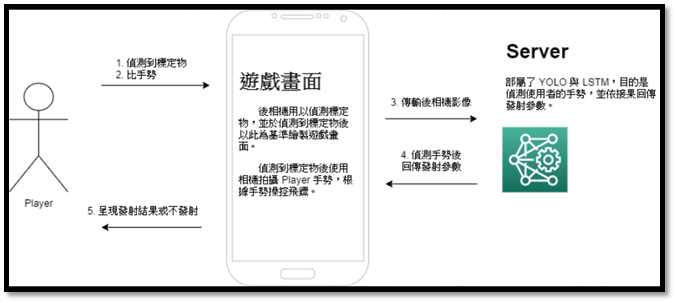
\includegraphics[width=10cm]{SYSTEM_Structure.png}
    \caption{系統架構示意圖}
    \label{fig:系統架構示意圖}
\end{figure}  
    
\section{報告組織}
本報告將系統分為前端、後端以及前後端傳輸,三大部分分別呈現介紹。前端會以使用到的技術著重進行介紹,分別為使用ARCore逕行標定物姿態估計,以及使用OpenGL ES繪製3D物件於螢幕上。前後端的傳輸將介紹如何使用UDP Socket傳輸後相機影像,以及玩家之間的資料傳遞的設計。後端執行手勢辨識運算,依序介紹SRCNN、手部物件辨識網路、LSTM三組神經網路架構,並將實驗過程與結果完整呈現。最後再分析實驗結果,並評估該組網路對於整體系統的優劣影響。

